\documentclass{beamer}
\usetheme{CambridgeUS}


% Title page details:
\title{GoTalk}
\author{Swasti \and Shreya \and Krishika \and Samridhi}
\date{\today}

\begin{document}

\begin{frame}
    \titlepage
    \centering HACKTIVISTS
\end{frame}

\begin{frame}{GO TALK}
    GoTalk is a real-time chat application designed to facilitate seamless communication among individuals or small groups.
\end{frame}

\section{Project Aim and Objectives}
\begin{frame}{Project Aim}
    \begin{itemize}
            \item To develop a real-time chat web application with chat history retrieval using Go, WebSocket and Firebase majorly
            \\ Our main aim is to Learn the Go language and Firebase and learn how to establish a client-server connection using WebSocket.
        \end{itemize}
\end{frame}

\section{Technologies and Tools Used}
\begin{frame}{Technologies and Tools Used}
    \begin{itemize}
        \item \textbf{Frontend:}
        \begin{itemize}
            \item HTML, CSS, JavaScript with Tailwind CSS for UI development.
        \end{itemize}
        \item \textbf{Backend:}
        \begin{itemize}
            \item Go (Golang) for server-side logic and WebSocket handling.
        \end{itemize}
        \item \textbf{WebSocket Library:}
        \begin{itemize}
            \item Gorilla WebSocket for WebSocket implementation in Go.
        \end{itemize}
        \item \textbf{Authentication and Database:}
        \begin{itemize}
            \item Firebase for real-time database and user authentication.
        \end{itemize}
        
    \end{itemize}
\end{frame}


%\begin{frame}{Objectives}
%    \begin{itemize}
%        \item \textbf{Seamless Real-time Communication:}
%        \begin{itemize}%
%            \item Enable instant messaging with minimal latency using WebSocket technology.
%        \end{itemize}
%       \item \textbf{Manage History Retrieval:}
%        \begin{itemize}%
%            \item Store and retrieve chat history to maintain continuity across sessions. 
%        \end{itemize}
%        \item \textbf{Secure User Authentication:}
%        \begin{itemize}
%            \item Implement robust authentication mechanisms to protect user data and ensure privacy. 
%        \end{itemize}
%    \end{itemize}
%\end{frame}

\section{Features and Functionalities}

\begin{frame}{Features and Functionalities}
    \begin{itemize}
        \item \textbf{Real-time Messaging:}
        \begin{itemize}
            \item Utilizes WebSocket for instant message delivery.
        \end{itemize}
        \item \textbf{User Authentication:}
        \begin{itemize}
            \item Integrated Firebase for secure user login and authentication.
        \end{itemize}
    \end{itemize}
\end{frame}

\begin{frame}{Features and Functionalities}
    \begin{itemize}
        \item \textbf{Message History:}
        \begin{itemize}
            \item Stores chat history in Firebase Realtime Database for seamless retrieval.
        \end{itemize}
        \item \textbf{User Interface:}
        \begin{itemize}
            \item Simple and intuitive design using HTML/CSS/JavaScript with Tailwind CSS for responsiveness.
        \end{itemize}
    \end{itemize}
\end{frame}

\begin{frame}{Database}
        \centering
        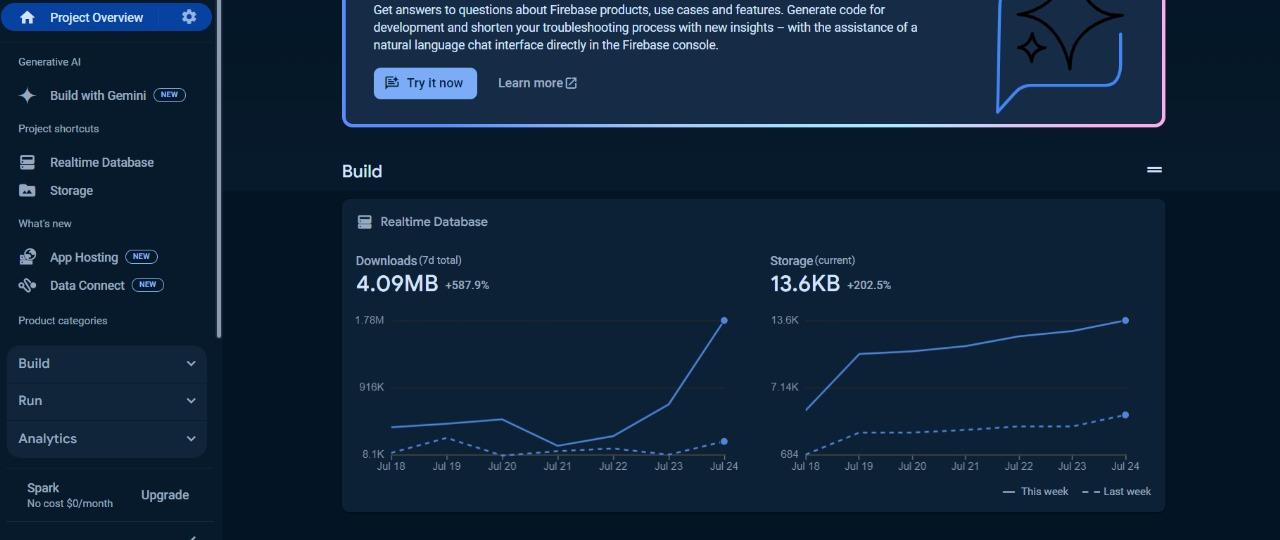
\includegraphics[width=\textwidth]{1.jpg}
\end{frame}

\begin{frame}{Database}
    \centering
    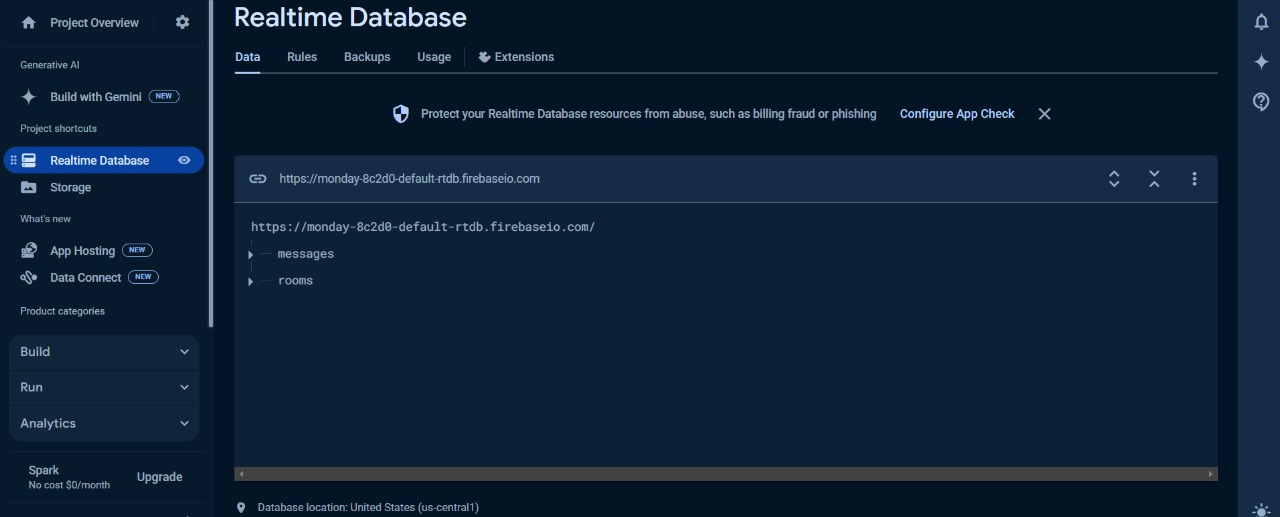
\includegraphics[width=\textwidth]{2.jpg}
\end{frame}

\begin{frame}{Database}
    \centering
    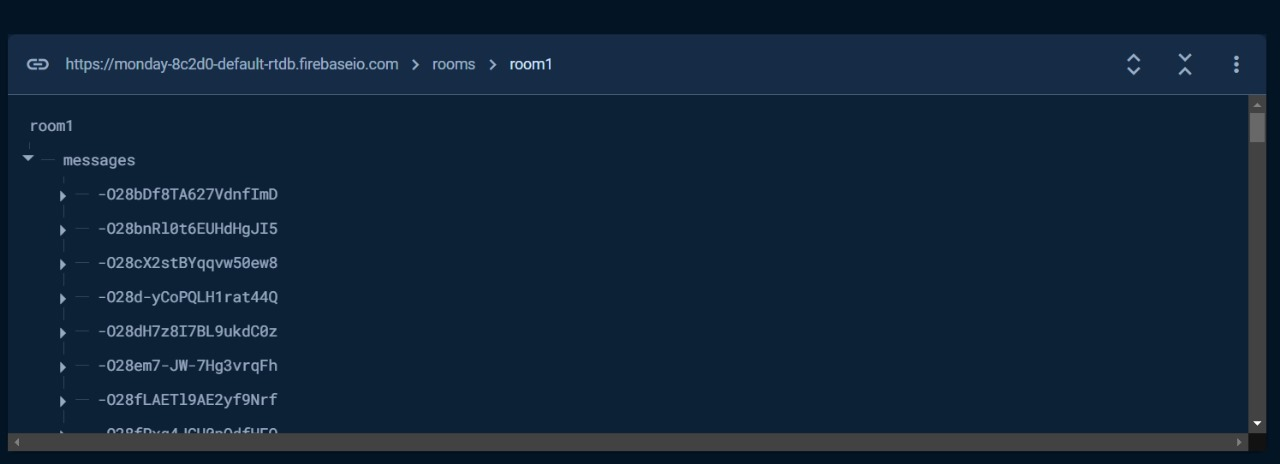
\includegraphics[width=\textwidth]{3.jpg}
\end{frame}

\begin{frame}{Database}
    \centering
    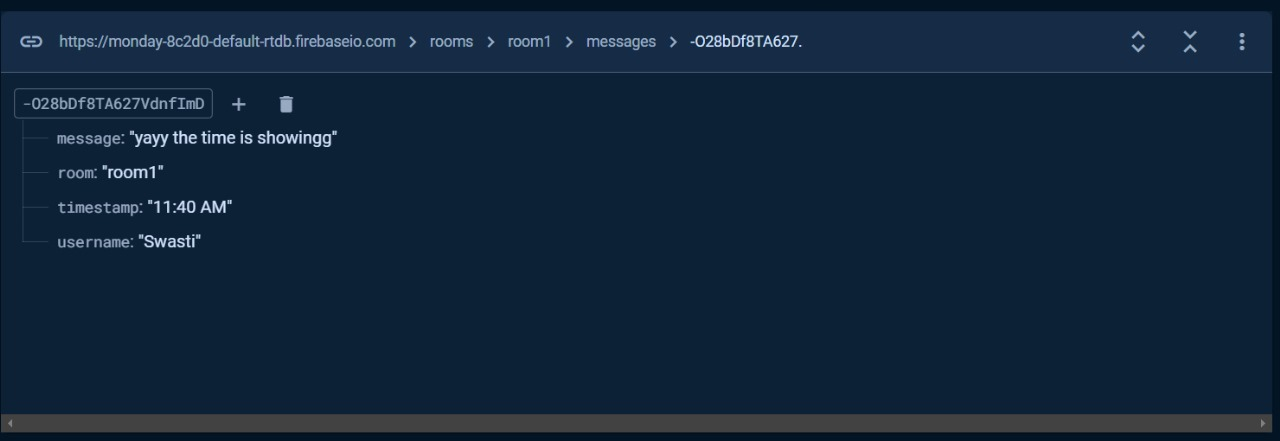
\includegraphics[width=\textwidth]{4.jpg}
\end{frame}

\section{Learnings}
\begin{frame}{Learnings}
    \begin{itemize}
        \item{We learnt working in teams.}
    \end{itemize}
    \begin{itemize}
        \item{We learned how to use git properly}
    \end{itemize}
    \begin{itemize}
        \item {Learned Go Language for backend development}
    \end{itemize}
    \begin{itemize}
        \item{WebSocket for enabling real-time communication}
    \end{itemize}
    \begin{itemize}
        \item{Firebase Realtime Database for storing chats and authentication}
    \end{itemize}
\end{frame}



\begin{frame}{Challenges Faced}
    \begin{itemize}
        \item{Implementing WebSocket Integration}
    \end{itemize}
    \begin{itemize}
        \item{Firebase Centralized Database}
    \end{itemize}
    \begin{itemize}
        \item{Cookie Management}
    \end{itemize}
    \begin{itemize}
        \item{Login Authentication}
    \end{itemize}
    
\end{frame}


\section{Conclusion}

\begin{frame}{Conclusion}
    \begin{itemize}
        \item Throughout this project, we faced and overcame several challenges, such as ensuring real-time synchronization, managing user sessions, and maintaining a responsive UI. Each challenge provided valuable learning experiences and contributed to the robustness of our final product.
    \end{itemize}
    \vfill
    \begin{center}
        \textbf{Thank you for your attention!}
    \end{center}
    \begin{center}
        Suggestions and Feedback welcomed.
    \end{center}
\end{frame}

\end{document}
